\documentclass{article}

\usepackage[utf8]{inputenc}
\usepackage{graphicx}


\title{Hello World}
\author{Ali}

\begin{document}
\maketitle

\begin{abstract}
This is my first abstract
\end{abstract}
Type your content here.

\begin{itemize}
\item first item
	\begin{itemize}
	\item first nested item
		\begin{itemize}
		\item second nested item
		\item second nested item
		\item second nested item
		\end{itemize}
	\item first nested item
	\item first nested item
	\end{itemize}
\item second item
\item third item
\end{itemize}
some texts some texts some texts some texts some texts some texts some texts some texts 

some texts some texts some texts some texts some texts some texts some texts some texts some texts 

\begin{enumerate}
\item first enumerate
	\begin{enumerate}
	\item first nested enumerate
	\item first nested enumerate
	\item first nested enumerate
	\end{enumerate}
\item first enumerate
\item first enumerate
\end{enumerate}

\textbf{Table:}

for each column we write a "c"

\begin{tabular}{ccc}
name & age & sex\\
ali & 29 & male\\
bita & 20& female
\end{tabular}

\textbf{Table with Horizontal line: }

\begin{tabular}{|c|l|r|}
\hline
name & age & sex\\
\hline
ali & 29 & male\\
\hline
bita & 20& female\\
\hline
\end{tabular}

\begin{center}
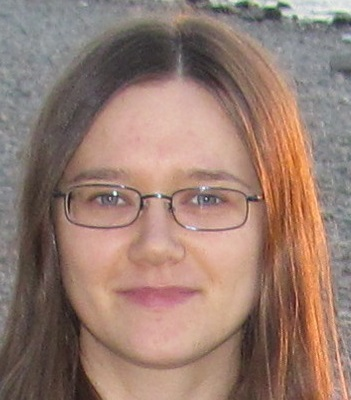
\includegraphics{{p/x1}} 
\end{center}

\includegraphics[scale=1.5]{{x1}}
hello again\\*
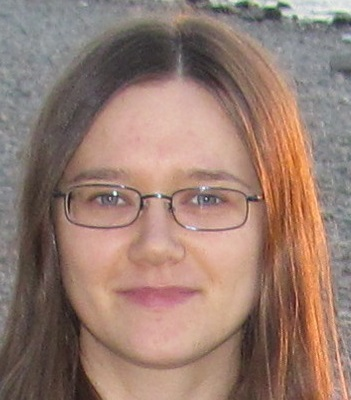
\includegraphics[angle=45,scale=0.75]{{p/x1}}
\\*

a sample on artificial intelligemce \cite{wenger2014artificial}.





\section{First Section}\label{secref 1}
this is the first section.
	\subsection{subsection 1}
	Hello from subsection 1
	\subsection{sub 2}
	Hello again
\section{Second Section} \ref{secref 1}
this is from second section with refrence
a sample on artificial intelligemce \cite{hwang1992potential}.

a sample on artificial intelligemce \cite{hwang}
\bibliographystyle{unsrt}
\bibliography{biblo}






\end{document}
